\documentclass{article}
\usepackage[utf8]{inputenc}
\usepackage[english]{babel}
\usepackage{graphicx}
\graphicspath{ {./images/} }
\usepackage[export]{adjustbox}
\usepackage[backend=biber,
style=ieee,
sorting=ynt]{biblatex}
\usepackage{csquotes}
\addbibresource{sources.bib}

\title{COMP 3613 Assignment 1}
\author{Half Moon Studios}
\date{November 2019}

\begin{document}

\maketitle
\vfill
Group Members:
\begin{itemize}
	\item []Selah Lewis 816012230 
	\item []Dominic Smart 816007605
	\item []Shereece A. A. Victor 816001671
	\item []Jerrel Williams 816009134
\end{itemize}

\newpage
\tableofcontents

\newpage
\section{Theory - Software Process}
\subsection{Software Performance Metrics (SPM) }


	
A software metric is a measure of software characteristics which are quantifiable or countable \cite{stacify}. Software metrics are important for many reasons, including measuring software performance, planning work items, measuring productivity, and many other uses \cite{stacify}.\\
   
   \begin{enumerate}
\item Apdex is a software metric measure which aims to quantify and measure the user satisfaction of a software application. The Apdex method converts various software metrics into a single number on a scale of 0 to 1, 0 being the lowest and 1, the highest. The formula can be seen below.\newline
       
       \begin{figure}[ht!]
       	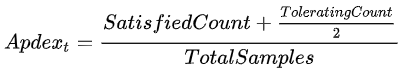
\includegraphics[width =0.8\textwidth, right]{images/sjGUFG.png}
       	\caption{Mathematical formula for Apdex}
       \end{figure}
       
       \item Response Time measures the server response of every single transaction or query. Response time starts when a user sends a request and ends at the time that the application states that the request has completed \cite{guru}. Average response time is the average of the response time measurements. The goal for software response time is 0.1 seconds with 1 second being the maximum upper limit, and most users will close the application if response time is greater than or equal to 6 seconds. Response time can be measured using applications such as JMeter and Load Runner.
       
        \item The Error Rate is a mathematical calculation which displays the percentage of problem requests against all requests \cite{guru}. Most errors, in the case of a web application, will be identified through the HTTP status codes returned by the server. However, some errors are not captured through that method and these errors must be accounted for separately. Errors also tend to raise in frequency as server load increases.

       
   \end{enumerate}
   \subsection{The Goal-Question-Metric Paradigm }
   The Goal-Question-Metric Paradigm is an approach used to measure software development in a hierarchical top down way.\\  
   At the highest level, the conceptual level, goals are defined. These include the business processes (eg., designing and testing software), products(eg., deliverables and documents), and/or resources(eg.,hardware and software used to produce output) which will be measured to assess performance according to the objectives of the organization.\cite{yahya2015using} \\
   Goals are then used to form questions which make up the operational level of the hierarchy.  These questions are used to determine how the goals can be achieved and which areas should be targeted. \\
   At the lowest level there are metrics, which are chosen to provide answers to one or many the questions to ensure that the metrics are collected from all viewpoints necessary. Metrics form the quantitative level and can be either subjective (eg., level of user satisfaction) or objective(eg., number of products sold). \cite{berander2006goal}\\
   \begin{figure}[ht!]
   	\includegraphics[width =1.2\textwidth, right]{images/GQM.png}
   	\caption{The hierarchical structure of the Goal Question Metrics Paradigm \cite{caldiera1994goal}}
   \end{figure}
   \newpage
   \subsection{The Five Stages in the Process change process}
   
    \begin{figure}[ht!]
   	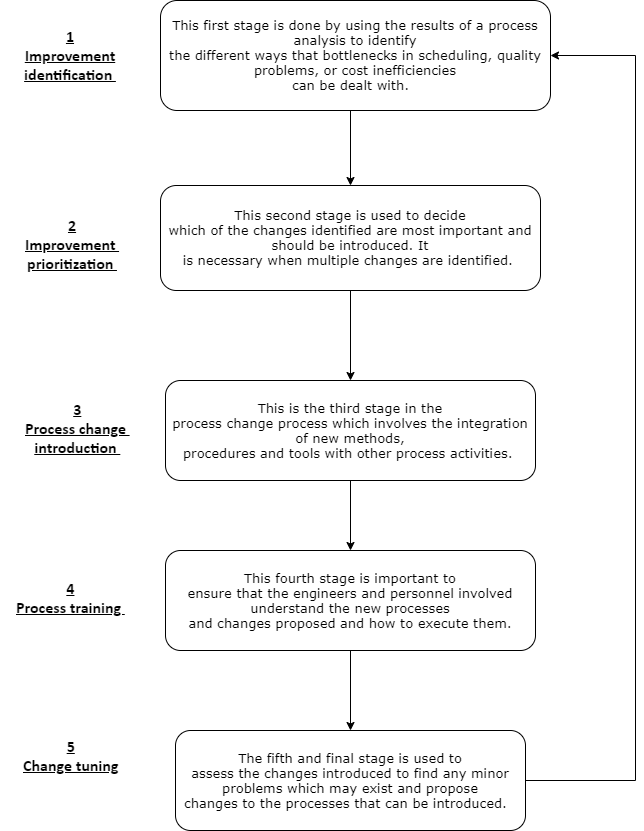
\includegraphics[width =\textwidth, ]{images/pcp.png}
   	\caption{The Five Stages in the Process change process \cite{pcp}}
   \end{figure}
\vfill
   
   \subsection{Process Improvement Models (PIMs)}
   Software Process Improvement Models aim to evaluate the software product, project, quality and drawbacks in order to streamline the software process.
   \begin{enumerate}
       

    \item The Capability Maturity Model involves a layered approach including 5 levels in order to refine the software development process. The first level is the initial level where processes are not sufficiently documented or replicable. Next is the repeatable level where organization has been developed and successes are now repeatable. After this is the defined level where a standard software processed has been developed. The managed level is next which is where the organization can now control and monitor its software processes. Finally is the optimizing level where software processes are constantly being improved through monitoring and feedback. An advantage of CMM is that higher CMM levels directly correlate to lower software defects. A disadvantage is that the level system of CMM is very rigid and may not tell a complete story.
    
    \item  Capability Maturity Model Integration is a process and behavioural model that helps optimize process improvement and decrease risks in development. CMMI also follows a level system which is the same as CMM but due to various improvements, it is more applicable in safety critical environments. An advantage of CMMI is that it fosters a mindset of quality maintenance within the programming team. A disadvantage is that while CMMI describes what process should be implemented by the organisation, it does not specify how. \cite{capability}
    
    \item Continuous Quality Improvement refers to identifying issues and solving them in a continuous cycle. It is a theory-based management system which focuses on processes and outcomes. An advantage of CQI is its flexibility, allowing the organization to quickly meet changing requirements. A disadvantage is the model’s difficulty of implementation as it requires an organization wide commitment to its practices.
    
    \item The Plan-Do-Check-Act model is a four-stage approach to continuously improving processes. It involves testing possible solutions, assessing results and implementing the successful solutions. The Plan phase involves identifying and analysing the problem. Do refers to testing the possible solution. Check is where the result is studied for effectiveness. Finally, Act is where the solution is implemented if the Check phase is passed. The advantage of PDCA is that it instils a mindset of continuous improvement which can improve efficiency and productivity over time. However, the disadvantage is that the PDCA cycle can be much slower than a straightforward solution implementation.\cite{plandocheckact}
    
    \item The ISO9000 model was defined as a set of standards for quality management and assurance to help document the quality systems necessary for an efficient organization. It is based on 7 quality management principles which can be applied to promote organizational improvement. These are, customer focus, leadership, engagement of people, process approach, improvement, evidence-based decision making and relationship management. Some advantages of ISO9000 are increased marketability, reduced operational expenses and improved internal communication. The disadvantage is that attaining ISO9000 certification can be quite costly due to the documentation and overhead requirements.
   \end{enumerate}
   


\newpage
\section{Software Engineering Tools and Requirements}
\subsection{Software Configuration Management (SCM)}

    Software Configuration Management is a systems engineering process aimed at establishing and maintaining consistency of a product’s performance, functional and physical attributes with its requirements, design, and operational information.\cite{tenbest} Some activities include:
    \begin{itemize}
        \item Promotion management (creating versions for developers)
        \item Release management (creating versions for clients)
        \item Branch management (managing concurrent developments)
    \end{itemize}

    However, these activities will employ the same software engineering tools and techniques used to create the product as illustrated below:\newline
  
    \begin{figure}[ht!]
    	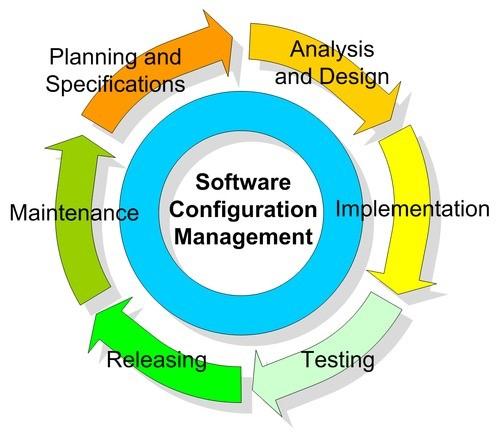
\includegraphics[width=0.8\textwidth, right]{images/cycle.jpg}
    	\caption{Showing the software configuration management cycle\cite{gcready}}
    \end{figure}
   
   \subsection{Assessing SaaS for Continuous Integration }
    Continuous integration refers to the automated building and testing of an application on every new commit. CircleCI is a Software as a Service model that delivers Continuous Integration to clients. Conversely, Jenkins is a self-contained Java based program used to achieve CI. One advantage of using CircleCI is that they will oversee the setup, security and maintenance of continuous integration instances. Hence, software firms can reap the benefit of quicker releases of higher quality/stable products without it being another administrative concern. \cite{contin}
\subsection{Requirements Tracing}
    Requirements Tracing refers to the ability to describe and follow the life of a requirement in both forward and backward directions. This entails tracing it from origins, through development, to deployment and through refinements. This is often achieved with a Requirements Traceability Matrix (RTM). It can be used to verify that all requirements have a corresponding design element, component, module or artefact. This is referred to as a forward trace. When the RTM is used to verify and document the source of the requirements, this is known as a backward trace. The backward trace is useful when customers have queries as to why certain features were included since it provides a comprehensive audit trail to make justified responses. Forward traceability is useful for checking the progress of the project by ensuring that each requirement is applied and tested thoroughly.\cite{reqtrac}


\newpage
\section{Theory - Software Design and Construction}

\subsection{Defensive Coding Practices} 

    Defensive Coding Practices:
    
    Defensive coding is a form of defensive design intended to ensure the continuing function of a piece of software under unforeseen circumstances. These are most often used in environments where high security, availability, or safety are required.\cite{adams_2017}
    Common defensive coding practices are \cite{hack2secure} - 
    \begin{enumerate}
    	\item Validation \newline
    	The basic premise behind the concept of input validation is “Do not trust without verifying.” Assume always you’re going to receive something you don’t expect. Two methods of validation are whitelisting and blacklisting.
    	
    	\item Code Access Security \newline
    	Code Access Security prevents the code from untrustworthy sources comprising run-time permissions to function privileged operations. It also prevents the code from the trusted sources against intentionally or unintentionally comprising the security.
    	
    	\item Container Versus Component\newline
    	Declarative security or container security offers a container managed strategy to ensure software flexibility, portability, and low deployment cost. Here, the security rules are configured outside the source code as a part of the deployment descriptor. The application container, or constraints, oversee applying dynamic security constraints to the code whereas programmatic or component security embeds the security rules in code or component itself. It involves a granular approach to implement security. When using this security, the programmatic enforcement is embedded in the application along with programmatic validation on policies to find, what a valid user is allowed to access. 
    	
    	\item Cryptographic Agility \newline
    	Cryptographic Agility is the capability of the code to switch to standard or recommended algorithms from insecure algorithms.
    	
    	\item Attack Surface Evaluation and Reduction \newline
    	The attack surface is defined as the various points where a hacker can get into the software and can achieve data access. The attack surface evaluation is the process of understanding the areas of risks in the software, to make security specialists and developers aware about the regions of software that are vulnerable to attacks and determine methods to reduce this.
    	
    	\item Memory Management \newline
    	Secure Memory Management can safeguard the revelation of data when it is processed. To implement proper memory management, it is important to follow some memory management concept. 
    \end{enumerate}

\subsection{Secure Coding}
    Secure Coding:
     
     Secure coding is the practice of developing computer software in a way that guards against the accidental introduction of security vulnerabilities. Defects, bugs and logic flaws are consistently the primary cause of commonly exploited software vulnerabilities.\cite{confluence}
\begin{enumerate}
    \item Validate input. Validate input from all untrusted data sources. 
    \item	Heed compiler warnings. Compile code using the highest warning level available for your compiler and eliminate warnings by modifying the code.
    \item	 Architect and design for security policies. Create software architecture and design your software to implement and enforce security policies. 
    \item	Keep it simple. Keep the design as simple and small as possible. Complex designs increase the likelihood that errors will be made in their implementation and use.
    \item	Default deny. Base access decisions on permission rather than exclusion. 
    \item	Adhere to the principle of least privilege. Every process should execute with the least set of privileges necessary to complete the job. Any elevated permission should only be accessed for the least amount of time required to complete the privileged task.
    \item	Sanitize data sent to other systems. Sanitize all data passed to complex subsystems such as command shells, relational databases, and commercial off-the-shelf components
    \item	Practice defense in depth. Manage risk with multiple defensive options, so that if one layer of defense turns out to be unreliable then another layer of defense can prevent a security flaw from becoming an exploitable vulnerability and limit the consequences of a successful exploit..
    \item	Use effective quality assurance techniques. Good quality assurance techniques can be effective in identifying and eliminating vulnerabilities. Fuzz testing, penetration testing, and source code audits should all be incorporated as part of an effective quality assurance program. 
    \item	Adopt a secure coding standard. Develop a secure coding standard for your target development language and platform.
\end{enumerate}	

 



 \subsection{Robust/Fault Tolerant Programs}
 Robust/Fault Tolerant Programs\\
Robustness describes an application's response to its input, while fault-tolerance describes an application's response to its environment. 

An app is robust when it can work consistently with inconsistent data. For example: a maps application is robust when it can parse addresses in various formats with various misspellings and return a useful location. A music player is robust when it can continue decoding an MP3 after encountering a malformed frame. 
An app is fault-tolerant when it can work consistently in an inconsistent environment. A database application is fault-tolerant when it can access an alternate shard when the primary is unavailable. A web application is fault-tolerant when it can continue handling requests from cache even when an API host is unreachable.

\newpage

\section{References}
\printbibliography[heading=none]

\end{document}


